\begin{frame}[t]
  \frametitle{Geometrie rozptylu}
  \vspace{.2em}
  \begin{itemize}
  	\item Anizotropní rozptyl v \textcolor{structure}{\emph{izotropním prostředí}} je vyjádřen funkcí \alt<1>{$\chi_s$}{\alert<2>{$\Sigma_s$}}:
  	\begin{overlayarea}{\textwidth}{2.35em}
  	\shorten{-.5em}{-.5em}
  	$$
  	  \alt<1>{
  	    \chi_s(\bomega'\ra\bomega) = \chi_s(\bomega\ra\bomega') = \chi_s(\bomega'\cdot\bomega) = \chi_s(\mu_0)
  	  }{
  	    \alert<2>{\Sigma_s(\br,\bomega'\ra\bomega)} = \Sigma_s(\br,\bomega\ra\bomega') = \Sigma_s(\bomega'\cdot\bomega) = \Sigma_s(\mu_0)
  	  },
  	$$
  	\lengthen
  	\end{overlayarea}
  	kde $\mu_0 = \cos \vartheta_0$ ~(kosinus rozptylového úhlu)\\[.5em]
  	
  	\only<1>{
      \centering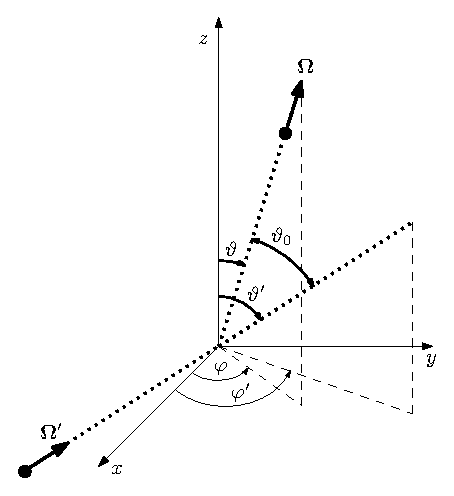
\includegraphics[scale=.75]{obr/scattering}
    }
  	\item<3->[$\Rabullet$] k popisu rozptylu nepotřebujeme zkoumat kartézský součin dvou sfér, nýbrž jen interval $[-1,1]$\\[1em]
  	\item<4-> V Hilbertově prostoru $\mathcal{H}([-1,1])$ můžeme funkci $\Sigma_s(\mu_0)$ ekvivalentně zapsat ve tvaru (zobecněného) Fourierova rozvoje vzhledem ke vhodné \alert<6>{úplné ortogonální bázi}
  	\item<5-> S jeho pomocí se budeme snažit vyjádřit \emph{\textcolor{structure}{rotačně invariantní}} operátor rozptylu $H$:
  	$$
  	  (H\angflux)(\br,\bomega) = \aintp{
        \Sigma_s(\br, \bomega'\cdot\bomega)
        \angflux(\br,\bomega')
      }
  	$$
  	ve finitní podobě (implementovatelné do počítače)
  \end{itemize}

\end{frame}

\begin{frame}
  \frametitle{Legendreovy polynomy}
  \vspace{-1em}
  \centering\includegraphics[height=.8\textheight]{obr/legendre}
  %\vspace{-1em}
  \begin{itemize}
  	\item \footnotesize $\P{0}(\mu) = 1,\ \ \P{1}(\mu) = \mu,\ \ \P{2}(\mu) = \frac12(3\mu^2 - 1),\ \ \P{2}(\mu) = \frac{1}{8} \left(3-30 \mu ^2+35 \mu ^4\right),\ \ \ldots$
  \end{itemize}
\end{frame}

\begin{frame}[t]
  \frametitle{Rozvoj do řady Legendreových polynomů}
  
  	  \centering$\Sigma_s(\br, \mu_0) = \suma[k]{0}{\infty}\frac{2k+1}{4\pi}\Sigma_{sk}(\br)\P{k}(\mu_0)$\\[.5em]
  	  
  \begin{itemize}	  
	  \item<2-> $\muint \P{j}(\mu)\P{k}(\mu) = \frac{2\delta_{jk}}{2k + 1}$\\[1em]
	  \item<2->[\Rabullet] $\Sigma_{sk}(\br) = 2\pi \muint[_0] \P{k}(\mu_0)\Sigma_s(\br, \mu_0)$
      \uncover<3->{\\[1em]
        $\Sigma_{s0}(\br) = \Sigma_s(\br)$\\[.5em]
   	    $\Sigma_{s1}(\br) = 2\pi \muint[_0] \mu_0\Sigma_s(\br, \mu_0)\uncover<4->{ = \muav(\br) \Sigma_s(\br)}$
   	    \begin{myitemize}
   	    	\item<4-> $ \muav(\br) = \frac{2\pi \muint[_0] \mu_0\Sigma_s(\br, \mu_0)}{2\pi \muint[_0] \Sigma_s(\br, \mu_0)} $~~\ldots~ 
   	    	\emph{střední kosinus rozptylových úhlů}\uncover<5>{\\[.5em]
   	    	$\big( = 2/(3A)$ pro elastický rozptyl na atomu s nukleonovým číslem $A\,\big)$}
   	    \end{myitemize}
   	}
  \end{itemize}

\begin{tikzpicture}[remember picture,overlay]  
  \node [xshift=-0.9cm,yshift=-1.1cm] at (current page.north east)
    {\includegraphics[width=1.5cm]{obr/Legendre.jpg}};
\end{tikzpicture}

\end{frame}

\begin{frame}
  \frametitle{Součtový vzorec}
\vspace{.75em}
\begin{overlayarea}{\textwidth}{\textheight}
\begin{itemize}
	\item Chceme vyjádřit
	  \alt<1-2>{
      $$
    	  (H\angflux)(\br,\alert<1-2>{\bomega}) = \aintp{
          \Sigma_s(\br, \bomega'\cdot\alert<1-2>{\bomega})
          \angflux(\br,\bomega')
        }
    	$$
   }{\\[1em]\hspace{1em}
      $
    	  (H\angflux)(\br,\alert<1-2>{\bomega}) = \aintp{
          \Sigma_s(\br, \bomega'\cdot\alert<1-2>{\bomega})
          \angflux(\br,\bomega')
        }
    	$
    	\vspace{0.75em}
   }
  \item<2-7> Zatím máme jen 
    \alt<1-2>{
      $$
        \Sigma_s(\br, \textcolor<2>{cyan}{\mu_0}) = \suma[k]{0}{\infty}\frac{2k+1}{4\pi}\Sigma_{sk}(\br)\P{k}(\textcolor<2>{cyan}{\mu_0})
      $$
      \vspace{-1.65em}
    }{\\[1em]\hspace{1em}
      $\Sigma_s(\br, \textcolor<2>{cyan}{\mu_0}) = \suma[k]{0}{\infty}\frac{2k+1}{4\pi}\Sigma_{sk}(\br)\P{k}(\textcolor<2>{cyan}{\mu_0})$
      \vspace{-.25em}
    }
    \alt<2-3>{
      \begin{align*}
	      \textcolor<2>{cyan}{\mu_0} &= \textcolor<2>{cyan}{\bomega'\cdot\bomega}
	      \uncover<3->{\\
      &= \lvect{\sint'\cosp',\sint'\sinp',\cost'}\!\cdot\!
	      \lvec{\sint\cosp,\sint\sinp,\cost}\\
      & = \mu'\mu + \sqrt{(1-\mu'^2)(1-\mu^2)}\cos(\azimuthal' - \azimuthal)\qquad\quad\qquad \big(\,\mu = \cos(\polar)\,\big)    
        }
      \end{align*}\vspace{-.5em}
    }{\\[1.25em] ale \vspace{-.25em}
      \begin{align*}
        \P{k}(\mu_0)
        &=P_k(\mu) P_k(\mu')+2 \sum _{m = 1}^k \frac{(k-m)!}{(k+m)!} \cos \bigl(m(\azimuthal - \azimuthal')\bigr) P_k^m(\mu) P_k^m(\mu')
        \uncover<5-7>{\\
        &=\frac{4\pi}{2k+1}\suma[m]{-k}{k}\textcolor<7>{blue}{\Y{k}{m}}(\alt<5>{\polar,\azimuthal}{\alert<6>{\bomega}})\textcolor<7>{blue}{\Yc{k}{m}}(\alt<5>{\polar',\azimuthal'}{\alert<6>{\bomega'}})
        }
      \end{align*}
    }
\end{itemize}
\end{overlayarea}

\begin{tikzpicture}[remember picture,overlay]  
  \alt<1-2>{
    \node [xshift=-0.9cm,yshift=-1.1cm] at (current page.north east)
      {\includegraphics[width=1.5cm]{obr/Legendre.jpg}};
  }{
    \node [xshift=-2.7cm,yshift=-3cm] at (current page.north east)
      {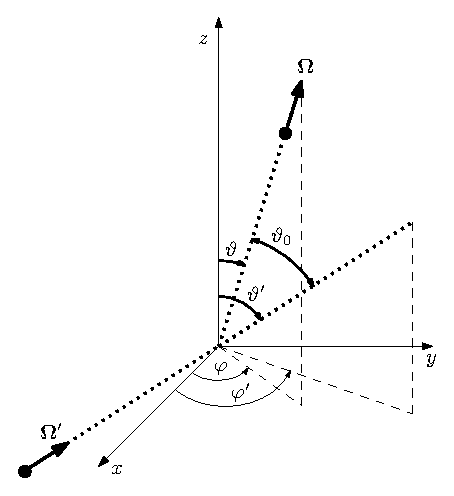
\includegraphics[width=5cm]{obr/scattering}};
  }
  \only<3->{
    \node [xshift=0.9cm,yshift=1.1cm] at (current page.south west)
      {\includegraphics[width=1.5cm]{obr/Legendre.jpg}};
  }
\end{tikzpicture}

\end{frame}

\begin{frame}
  \frametitle{Sférické harmoniky}
  \framesubtitle{Definice}
  \begin{itemize}
  	\item<1-3> Sférická harmonická funkce \textcolor{structure}{\emph{řádu $m$}} a \textcolor{structure}{\emph{stupně $l$}}
  	  \begin{gather*}
        \Y{l}{m}(\bomega) = \Y{l}{m}(\alt<1>{\polar}{\mu},\azimuthal) = \sqrt{\frac{2l+1}{4\pi}\frac{(l-m)!}{(l+m)!}} \P{l}^m(
          \alt<1>{\cos\polar}{\mu}
        )e^{i m \azimuthal}\\[.5em]
        \alt<1>{\polar\in [0,\pi]}{\mu\in[-1,1]},\ \azimuthal\in [0,2\pi),\quad 
        l\in\mathbb{N}_0,\ m\in\mathbb{Z},\ 0\leq m \leq l
      \end{gather*}
    \item<3> \textcolor{structure}{\emph{Přidružené Legendreovy funkce}} (\emph{Associated Legendre functions})
    $$
      \P{l}^m(\mu) = 
      \begin{cases} 
        (-1)^m\sqrt{(1-\mu^2)^m}\ \der[m]{\P{l}(\mu)}{\mu} & \hphantom{-}\,0 \leq m \leq l,\\[1em]
        \displaystyle (-1)^{-m}\,\frac{(l+m)!}{(l-m)!}\P{l}^{-m}(\mu) & -l \leq m < 0 
      \end{cases}
    $$
  \end{itemize}
  
\begin{tikzpicture}[remember picture,overlay]  
  \node [xshift=-1cm,yshift=-0.8cm] at (current page.north east)
    {\includegraphics[width=1.75cm]{obr/harmoniky.png}};

   \only<4>{ 
     \node [anchor=center,yshift=-0.8cm] at (current page.center)
       {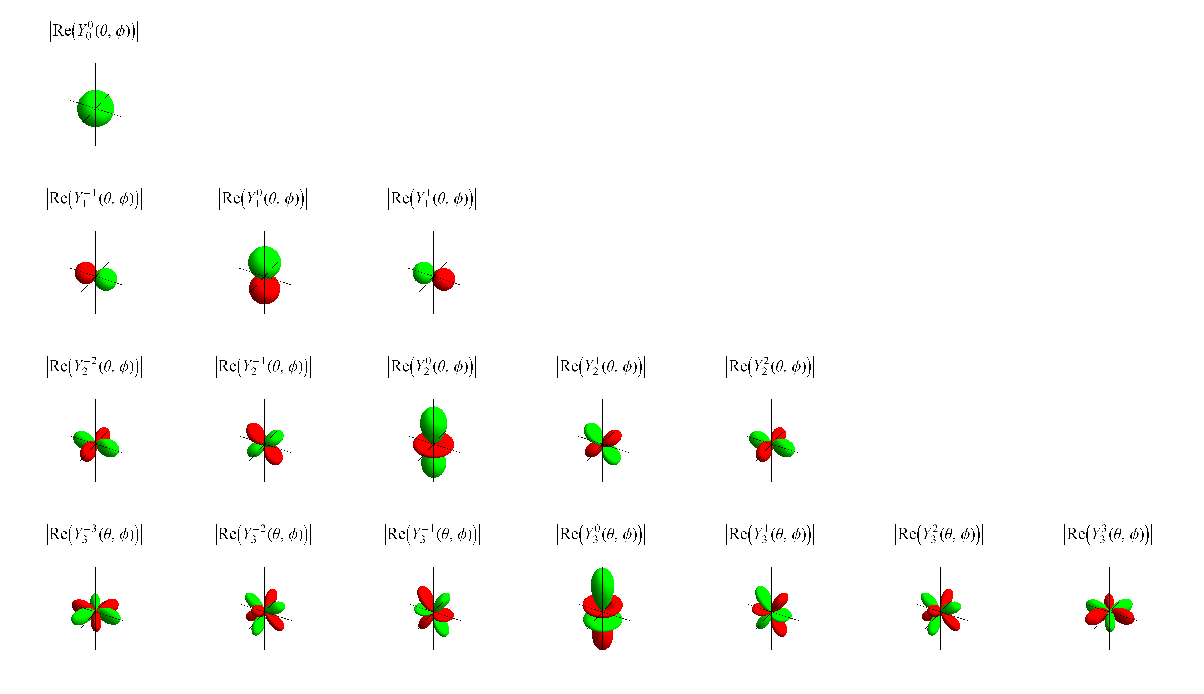
\includegraphics[width=1.05\textwidth]{obr/sh}};
   }
\end{tikzpicture}

\end{frame}

\begin{frame}
  \frametitle{Sférické harmonické funkce}
  \framesubtitle{Vlastnosti}
  \begin{itemize}
  	\item Úplný ortonormální systém na sféře vzhledem ke skalárnímu součinu
  	  $$
        \aint{\Y{l}{m}(\bomega)\Yc{l}{m}(\bomega)}
        = \int_{0}^{2\pi}\d{\azimuthal}\int_{-1}^{1}\d{\mu}
        \Y{l}{m}(\mu,\azimuthal)\Yc{l'}{m'}(\mu,\azimuthal)
      $$
    \item SHF stupně $l$ generují rotačně invariantní podprostor $\Lp{2}(\SS)$:
      $$\Lambda_l = \mathrm{Span}\bigl\{\Y{l}{m}; -l \leq m \leq l\bigr\},$$
    takový, že $R(\Lambda_l) \subset \Lambda_l$ pro libovolnou rotaci $R$
    \begin{itemize}
    	\item<2-> vlastní prostor příslušný $l$-tému vl. č. Laplaceova-Beltramiho
    operátoru $\nabla\cdot(\nabla)$ na sféře
      \item<3-> \alert{vlastní prostor libovolného rotačně invariantního operátoru}
    \end{itemize}
    
    \item<4-> Lze je použít pro zobecněný Fourierův rozvoj (tzv. \emph{Laplaceův rozvoj})
    funkcí def. na sféře -- 3D analogie rozvoje pomocí trigon. polynomů
    \item<5-> Azimutálně symetrické (nezávislé na $\azimuthal$ SHF: Legendreovy polynomy
   
  \end{itemize}
\end{frame}

\begin{frame}
  \frametitle{Sférické harmonické funkce}
  \framesubtitle{Použití -- reprezentace operátoru rozptylu}
  
  \begin{itemize}
  	\item Zobecněný Fourierův rozvoj rotačně invariantního operátoru rozptylu
  	do řady jeho vlastních funkcí
  \end{itemize}
\begin{align*}
\alert<6>{(H\angflux)(\br,\bomega)} &= 
  \aintp{
    \Sigma_s(\br, \bomega'\cdot\bomega)
    \angflux(\br,\bomega')
  }\uncover<2->{\\
& = \aintp{
      \suma[k]{0}{\infty}
        \frac{2k+1}{4\pi}\Sigma_{sk}(\br)\P{k}(\bomega'\cdot\bomega)
        \angflux(\br,\bomega')
    }\uncover<3->{\\
& = \aintp{
      \suma[k]{0}{\infty}
	      \Sigma_{sk}(\br)\suma[m]{-k}{k}\Y{k}{m}(\bomega)\Yc{k}{m}(\bomega')
        \angflux(\br,\bomega')
    }\uncover<4->{\\
& = \suma[k]{0}{\infty}
	    \Sigma_{sk}(\br)\suma[m]{-k}{k}\Y{k}{m}(\bomega) \aintp{
	      \Yc{k}{m}(\bomega')\angflux(\br,\bomega')
	    }\uncover<5->{\\
& \alert<6>{= \suma[k]{0}{\infty}
      \Sigma_{sk}(\br)\suma[m]{-k}{k}\Y{k}{m}(\bomega)\angmomgen{k}{m}(\br)}
}}}}
\end{align*}

\end{frame}

\begin{frame}
  \frametitle{Sférické harmonické funkce}
  \framesubtitle{Použití -- reprezentace operátoru rozptylu}
  
  \centering \alert<1>{$(H\angflux)(\br,\bomega) = \suma[k]{0}{\infty}\Sigma_{sk}(\br)\suma[m]{-k}{k}\Y{k}{m}(\bomega)\alert<2>{\angmomgen{k}{m}(\br)}$}
  
  \begin{itemize}
  	\item<2-> \alert<2>{$\angmomgen{k}{m}(\br) = \aint{\Yc{k}{m}(\bomega)\angflux(\br,\bomega)}$}\vspace{.5em}
  	\begin{itemize}
  		\item[\ldots]	  koeficienty zobecněného Fourierova rozvoje $\angflux(\br,\bomega)$ vzhledem k $\bomega$:
  		  \vspace{-.5em}
    		  \begin{equation*}
    		    \angflux(\br,\bomega) = \suma[k]{0}{\infty}\suma[m]{-k}{k}\angmomgen{k}{m}(\br)\Y{k}{m}(\bomega)
    		  \end{equation*}
   	\end{itemize}
    \item<3-> Finitní reprezentaci operátoru rozptylu získáme použitím konečného rozvoje ($0 \leq k \leq L < \infty$):
    \begin{myitemize}
    	\item rozptylovací charakteristiku každého materiálu uchováváme v podobě pole příslušných koeficientů $\Sigma_{sk}$
    \end{myitemize}
  \end{itemize}

\end{frame}

\begin{frame}
  \frametitle{Sférické harmonické funkce}
  \framesubtitle{Použití -- metoda $P_L$}
  
  \begin{itemize}
  	\item  Rozvoj 
  	  \begin{equation*}
		    \angflux(\br,\bomega) = \suma[k]{0}{L}\suma[m]{-k}{k}\angmomgen{k}{m}(\br)\Y{k}{m}(\bomega)
		  \end{equation*}
		  pro $L < \infty$ lze použít přímo k definici přibližného řešení LBR:
		  \begin{myitemize}
		  	\item dosazením rozvoje do LBR, použitím rozvoje operátoru rozptylu z předchozích slajdů a 
		  	  aplikací Galerkinovy metody vzhledem ke směrové proměnné získáme soustavu PDR 1. řádu 
		  	  v prostorové proměnné
		  	\item řešením vzniklé úlohy obdržíme $\angmomgen{k}{m}(\br)$, a tedy i $\angflux(\br,\bomega)$
		  \end{myitemize}
  \end{itemize}
  \uncover<2>{
\vspace{1em}
  \begin{center}
    {\huge  \textcolor{blue}{\emph{ O tom ale zas až někdy příště ...} ;-)}}
  \end{center}
  }
\end{frame}
